\chapter{Proposed Methods}
\label{chap3:proposed_methods}

The present chapter provides an extensive overview of two methods that try to explain whether two images from periocular regions come from the same person or not. To that end, the remainder of this chapter is organised as follows: sections \ref{sec:chap3_method_a} and \ref{sec:chap3_method_b} contain an overview of the methods that were developed, while section \ref{sec:chap3_conclusion} summarises the main takeaways from the present chapter.

\section{Deep Adversarial Framework for Visually Explainable Periocular Recognition}
\label{sec:chap3_method_a}

The first framework, that set out to tackle the problem of periocular recognition, is based on widely used \ac{DL} architectures: \ac{CNN}s and \ac{GAN}s. Such models were used as the basis of both parts that make up the final answer: the \ac{CNN} for the traditional binary part and the \ac{GAN} for the visual counterpart. To go over the details of said method, subsection \ref{subsec:chap3_method_a_data_preprocessing} covers the pre-processing steps that enabled the subsequent stages, which are later described in subsection \ref{subsec:chap3_method_a_description}.

\subsection{Data Pre-processing}
\label{subsec:chap3_method_a_data_preprocessing}

The data pre-processing stage is quite common in pipelines that involve some kind of \ac{DL} model. These models often demand fixed size inputs and perform optimally with balanced and rich datasets. Naturally, the present method also required some preliminary steps:

\begin{figure}[H]
\centering
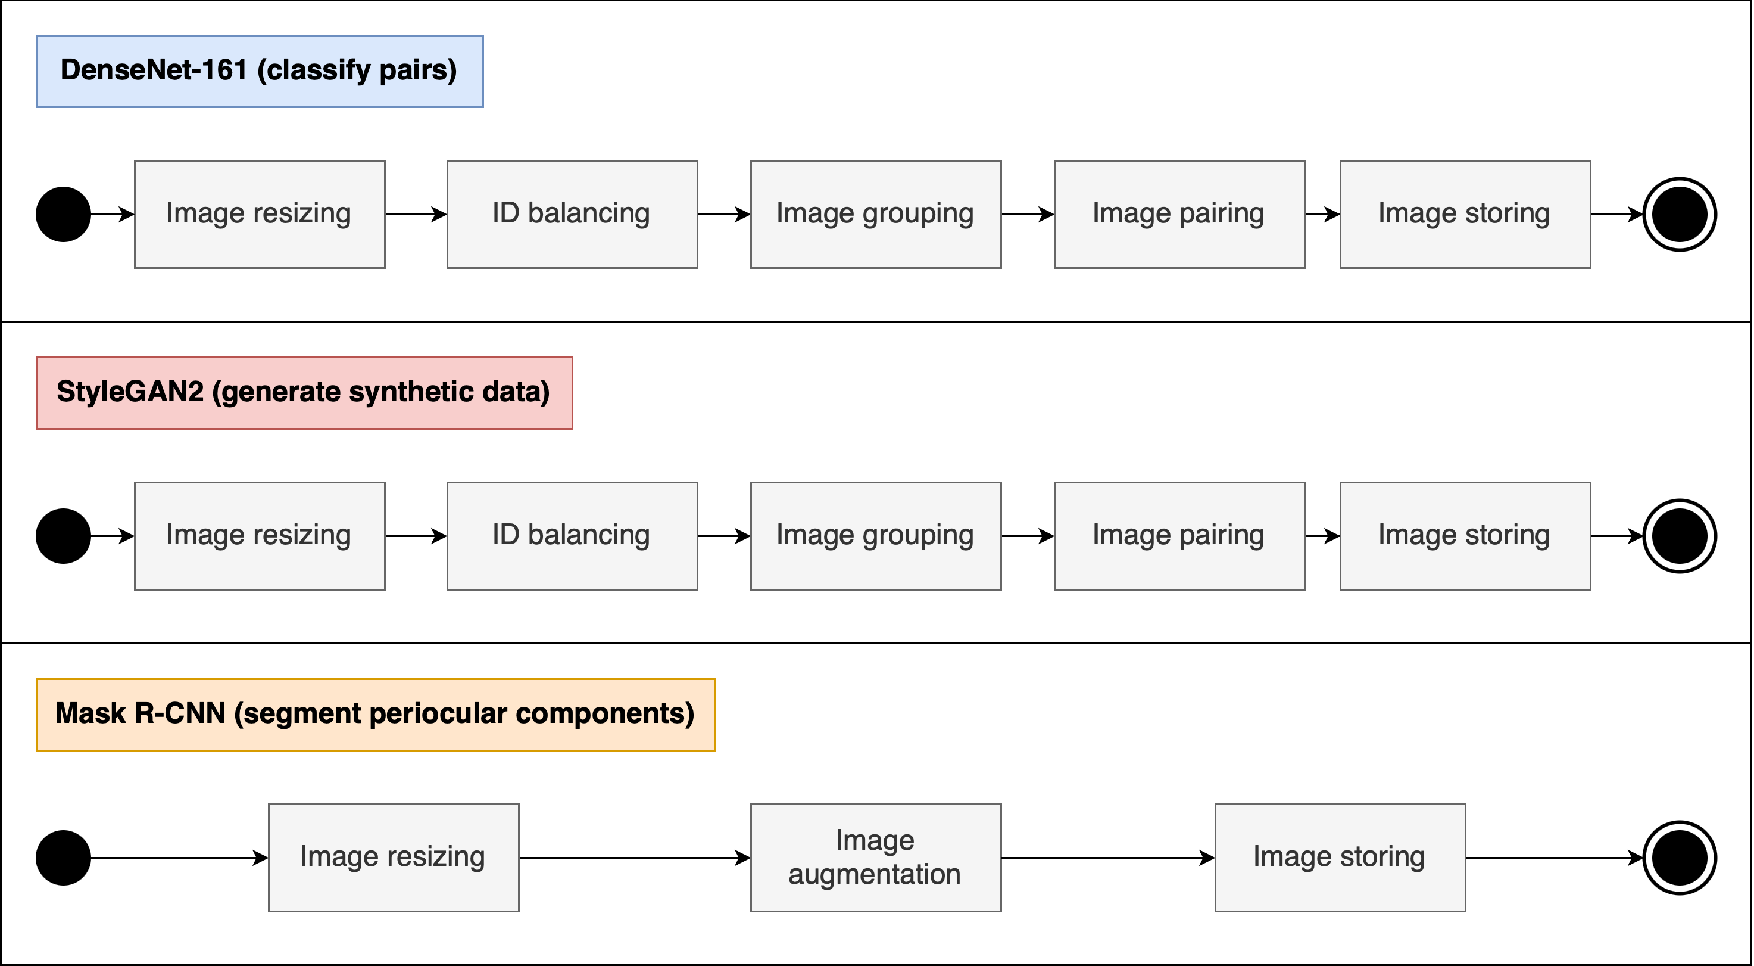
\includegraphics[width=370pt]{figures/figure_26.pdf}
\caption{Diagram of the data pre-processing pipeline. The images are resized, processed and stored in proper folders.}
\label{fig:method_a_data_pre_processing_diagram}
\end{figure}

Fig. \ref{fig:method_a_data_pre_processing_diagram} depicts three major sets (one for each of the main components):

\begin{itemize}
    \item \textbf{Image resizing}: the images are resized to a fixed size (e.g., $256$x$256$ pixels).
    \item \textbf{ID balancing}: considering that, in the unprocessed dataset, some IDs possess more images than others, each ID gets it images either sampled or augmented. On one hand, if the ID has less images than a pre-defined target, the existing ones are augmented to reach said target (with techniques like horizontal flips, rotations, contrast changes or noise additions). On the other hand, if the image count is too great, a simple sampling routine chooses as many images as the target value enforces.
    \item \textbf{Image grouping}: the images are grouped by ID and some of them are reserved just for the test phase (according to a pre-established set).
    \item \textbf{Image pairing}: the images are paired with each other, to form either "genuine" or "impostor" pairs.
    \item \textbf{Image storing}: the images are stored in folders targeted towards training, validation and testing (in the case of DenseNet). As obviously required for the \ac{CNN} and \ac{GAN}, within each of these main folders there are class sub-folders ("$0$" for "impostor" pairs and "$1$" for "genuine" pairs). The Mask \ac{R-CNN} model just required the images and corresponding masks to be stored in standard folders.
\end{itemize}

\subsection{Method Description}
\label{subsec:chap3_method_a_description}

\begin{figure}[H]
\centering
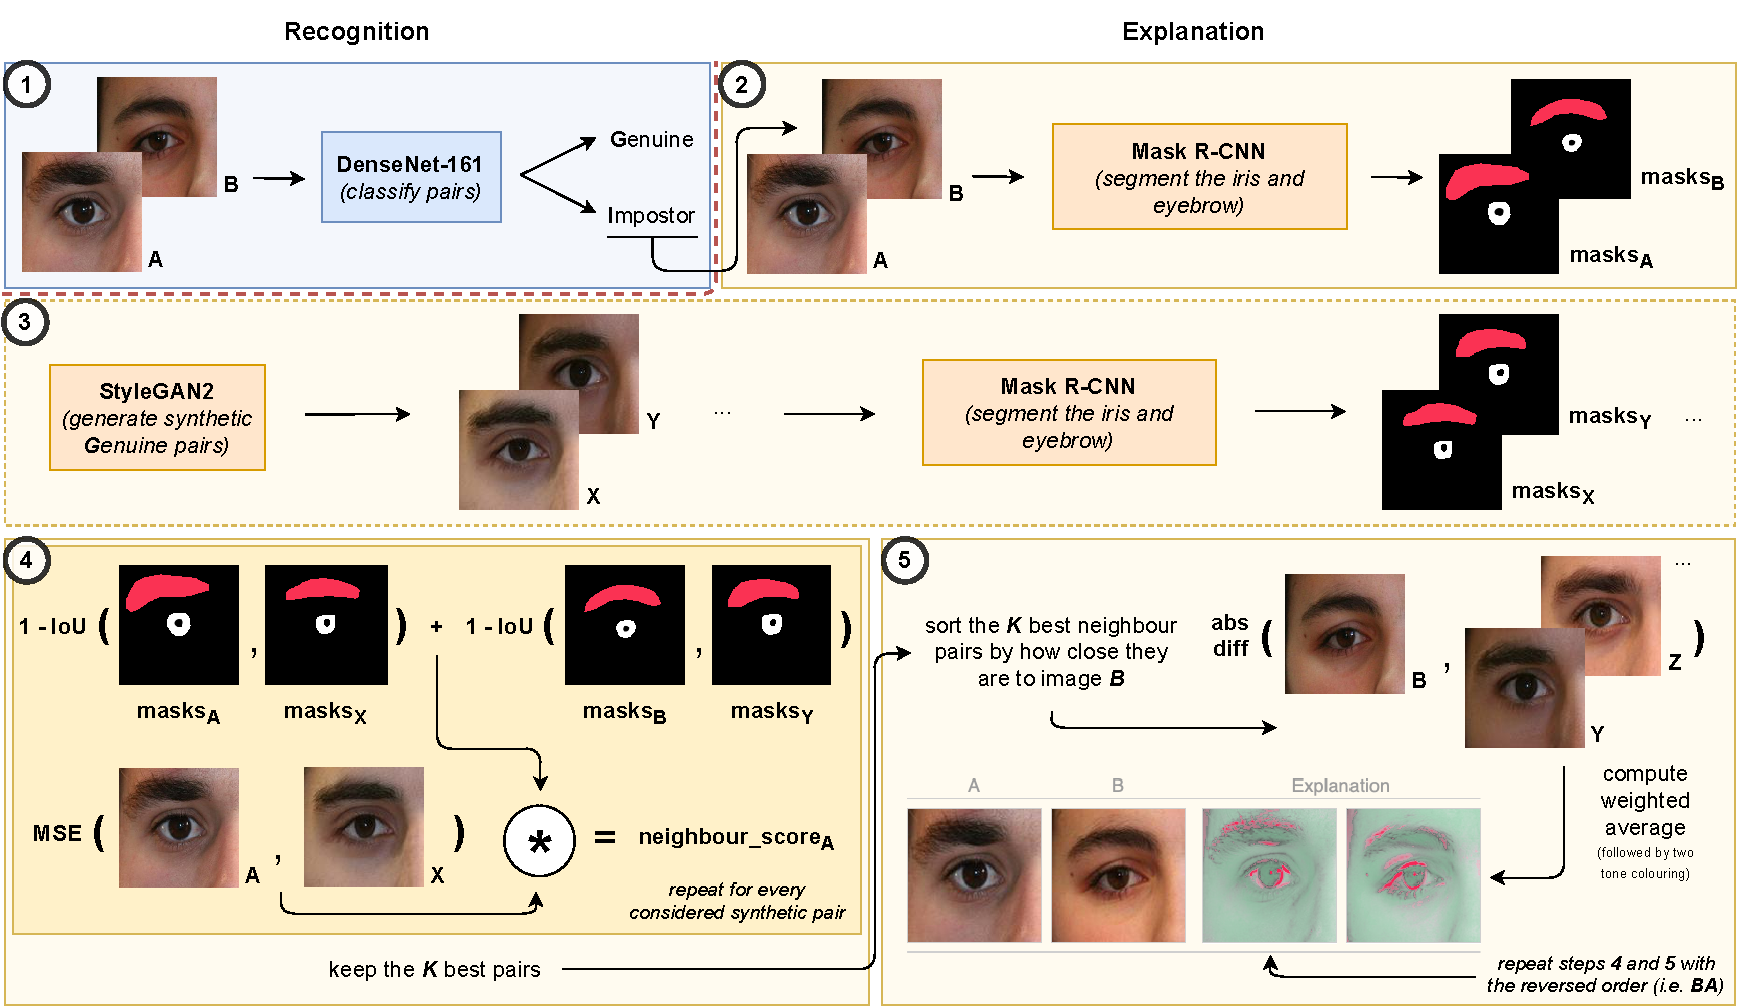
\includegraphics[width=\textwidth]{figures/figure_27.pdf}
\caption{Cohesive perspective of the main pipeline of the proposed solution. The recognition step encompasses a \ac{CNN} that distinguishes between ''genuine'' and ''impostor'' pairs. Then, upon an ''impostor'' decision, steps two to five (explanation) find the $k$ ''genuine'' synthetic pairs amongst a large set that most closely resemble the query pair. Assuming the alignment between the query and the retrieved pairs, the element-wise differences between the query and a weighted average of the retrieved elements provides a visual explanation of the features in the query that would have to be different to turn it into a ''genuine'' pair.}
\label{fig:method_a_main_diagram}
\end{figure}

\subsubsection{Learning Phase}
\label{subsec:chap3_method_a_learning_phase}

The main components of the proposed method comprise three well known models: the DenseNet-$161$, Mask \ac{R-CNN} and Style\ac{GAN}$2$. The first one (DenseNet-$161$) is trained to solve an identity verification problem, while the segmentation model (Mask \ac{R-CNN}) is fine-tuned to produce high-quality masks for the iris and eyebrow. Finally, the \ac{GAN} model (Style\ac{GAN}$2$) learns how to create synthetic data that, while closely resembling the distributions in the training set, is diverse enough to approximate unseen subjects. Additionally, a fourth, auxiliary model (ResNet-$18$) is fitted to discriminate between images from the left and right sides of the face. Although trained separately, all the models learn from the same training split, which excludes a set of disjoint IDs that are reserved for performance evaluation purposes.

Regarding the model used in the verification task (DenseNet-$161$), it should be stated that it has much more parameters than the network used by Zhao and Kumar~\cite{accurate_periocular_recognition} in their solution. This might be the fact that sustained slightly better recognition performance of our model with respect to the baseline (subsection \ref{subsec:chap4_recognition_accuracy_evaluation}), but also at the expense of a substantial higher computational cost of classification than the baseline, which might be impracticable in some cases.

\subsubsection{Inference Phase}
\label{subsec:chap3_method_a_inference_phase}

Once trained, our method is conceptually divided into five major steps, as depicted in Fig. \ref{fig:method_a_main_diagram}. Firstly, the DenseNet-$161$ model is used to verify the claimed identity: upon receiving a pair of images, the model discriminates  between ''genuine''/''impostor'' pairs. If the pair is deemed to be ''impostor'', the remaining steps create a visually accurate explanation of that decision.

The second step takes the query pair and, using Mask \ac{R-CNN}, segments the irises and eyebrows regions. Next, step three uses the Style\ac{GAN}$2$ generator to create a large, synthetic set of exclusively ''genuine'' pairs (i.e., where both images belong to the same person). For each of these synthetic pairs, the ResNet-$18$ model determines its side configuration (i.e., whether images regard the left or right side of the face) and, as before, masks are obtained by the segmentation model. Uncurated synthetic samples are shown in Fig. \ref{fig:synthetic_samples}.

After obtaining the synthetic data and their corresponding masks, the synthetic dataset is indexed based on the coordinates of the center of the iris, which will enable faster search in the retrieval step. To that end, the clustering algorithm K-Means is trained on a subset of the iris segmentation masks to obtain three centroids, one for each major iris gaze family (i.e., left, centre and right). This way, we index the available pairs based on their combination of iris positions (e.g., left-left, right-centre, \ldots). By doing so, when searching, we can just rely on the synthetic pairs that share the same combination as the test pair, saving time and useless calculations. 

\begin{figure}[H]
\centering
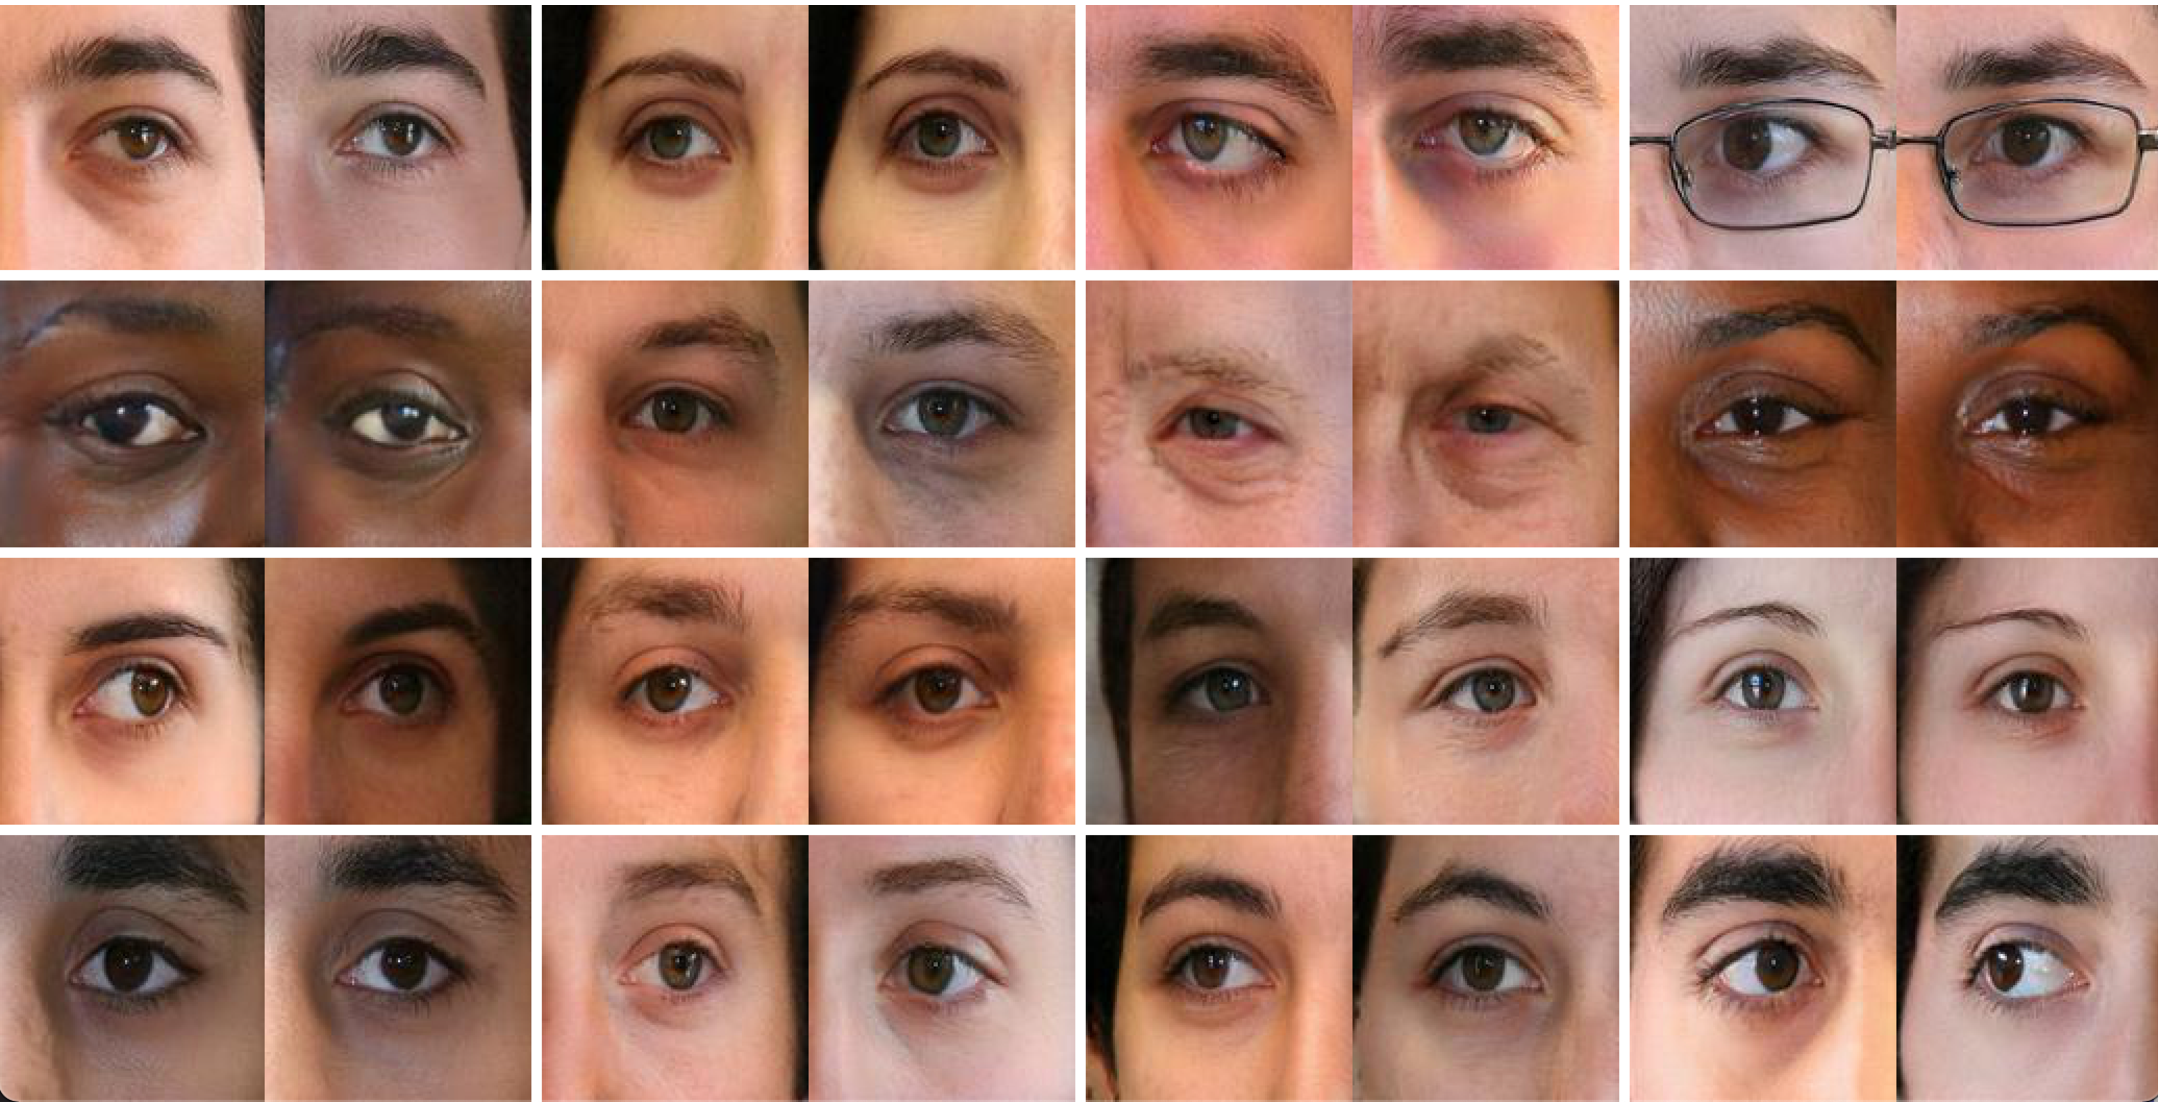
\includegraphics[width=0.9\textwidth]{figures/figure_28.pdf}
\caption{Examples of the synthetic image pairs in our dataset, generated according to a \ac{GAN} model. These elements are drawn exclusively from the ''genuine'' distribution. Upon  a query, the most similar synthetic pairs with respect to the query are found, which will provide the features/regions that would transform the query into a ''genuine'' comparison.}
\label{fig:synthetic_samples}
\end{figure}

Upon settling for a portion of the synthetic dataset that closely meets the iris position constraint, the segmentation masks are further used to determine which synthetic pairs have the iris and eyebrow approximately overlapped to the query. This is an important requirement to obtain visually pleasant explanations, given that pixel-wise differences are extremely sensitive to differences in phase (i.e., component misalignment). Accordingly, we obtain a similarity score $s_X$ between each synthetic neighbour and the query, given by:
\begin{equation}
    s_X = \omega_{\text{masks}} * ||\text{query}_{\text{A}} - \text{neighbour}_{\text{X}}||_2,
\label{eq:neighbour_score}
\end{equation}
being $||.||_2$ the $\ell-2$ norm and $\omega_.$ a weight that considers component misalignment. This way, we obtain a weighted distance between each synthetic neighbour and the first image of the query pair. $\omega_{\text{masks}}$ values serve to favour pairs that have good alignment, considering $1 - \text{IoU}(.,.)$, i.e., the complement of the \ac{IoU} of the synthetic/query segmentation masks. 

In practice, we search amongst the (large) thousands of synthetic pairs for the closest to the query pair in terms of the first image. Therefore, given that the second image of the query pair is from a different subject, it will most likely have features that are different to the synthetic neighbours, which are exactly the kind of dissimilarities that make up the final explanations.
This way, the $K$ closest neighbours are sorted according to their element-wise distance to image $B$, using  (\ref{eq:neighbour_score}). 

Finally, to produce the visual explanation, the $K$ best neighbours are used to obtain the pixel-wise differences against the query pair image $B$. In practice, a neighbour distance is subtracted from the total sum of distances, creating an inverted distance. This assures that the contribution of the closest synthetic neighbours to the final result is more important than of those with bigger distances. 

\subsubsection{Implementation Details}
\label{subsec:chap3_method_a_implementation_details}

The DenseNet-$161$ model was trained for $15$ epochs with a learning rate of $0.0002$ and a batch size of $64$ image pairs. The Adam algorithm was used for the weight optimisation process (with default $\beta_1$ and $\beta_2$ values). A similar training setup was used to train the ResNet-$18$ model, albeit for a smaller number of epochs (i.e., $5$).

For the Mask \ac{R-CNN}'s training process, we kept its default values, using a learning rate of $0.001$, a batch size of $1$ and $30$ epochs worth of training (in this case, fine-tuning from the COCO pre-trained weights).

Regarding the Style\ac{GAN}$2$ architecture, the training step comprised a total of $80 000$ iterations and a batch size of $8$. After converging, the generator is capable of synthesising realistic looking images, such as the roughly $400 000$ pairs that make up the artificial dataset. Finally, for the number $K$, that determines how many synthetic neighbours should be kept, we used a default value of $15$.

\section{Automatic Generation of Image Captions}
\label{sec:chap3_method_b}

For the second method considered in the scope of this dissertation, the feature extraction prowess of a  \ac{CNN} and the text generation of an \ac{LSTM} were combined to allow for automatic image captioning. The basic premise is that this solution takes as input an image pair and produces text descriptions in which, hopefully, the different periocular components are highlighted. As before, subsection \ref{subsec:chap3_method_b_data_preprocessing} describes the data preparation steps, while subsection \ref{subsec:chap3_method_b_description} describes the main architecture.

\subsection{Data Pre-processing}
\label{subsec:chap3_method_b_data_preprocessing}
This admittedly simpler method also required some preliminary steps, to ensure proper sizing and storing of the image pairs:

\begin{figure}[H]
\centering
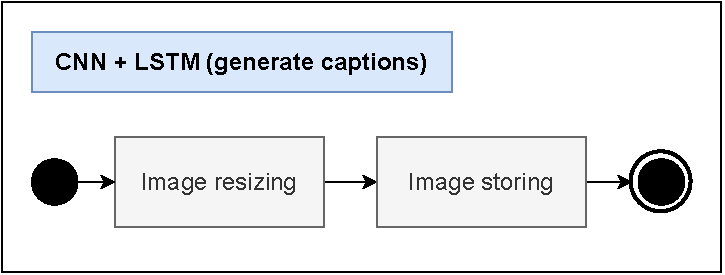
\includegraphics[width=250pt]{figures/figure_29.pdf}
\caption{Diagram of the second method's pre-processing pipeline. The images are resized and stored in proper folders.}
\label{fig:method_b_data_pre_processing_diagram}
\end{figure}

As Fig. \ref{fig:method_b_data_pre_processing_diagram} depicts it, the image pairs are resized to the pre-established size required by the ResNet model (i.e., $224$x$224$ pixels) and stored in a simple folder. Then, once in the training stage, the images and captions are adequately paired.

\subsection{Method Description}
\label{subsec:chap3_method_b_description}

\subsubsection{Learning Phase}
\label{subsec:chap3_method_b_learning_phase}

\begin{figure}[H]
\centering
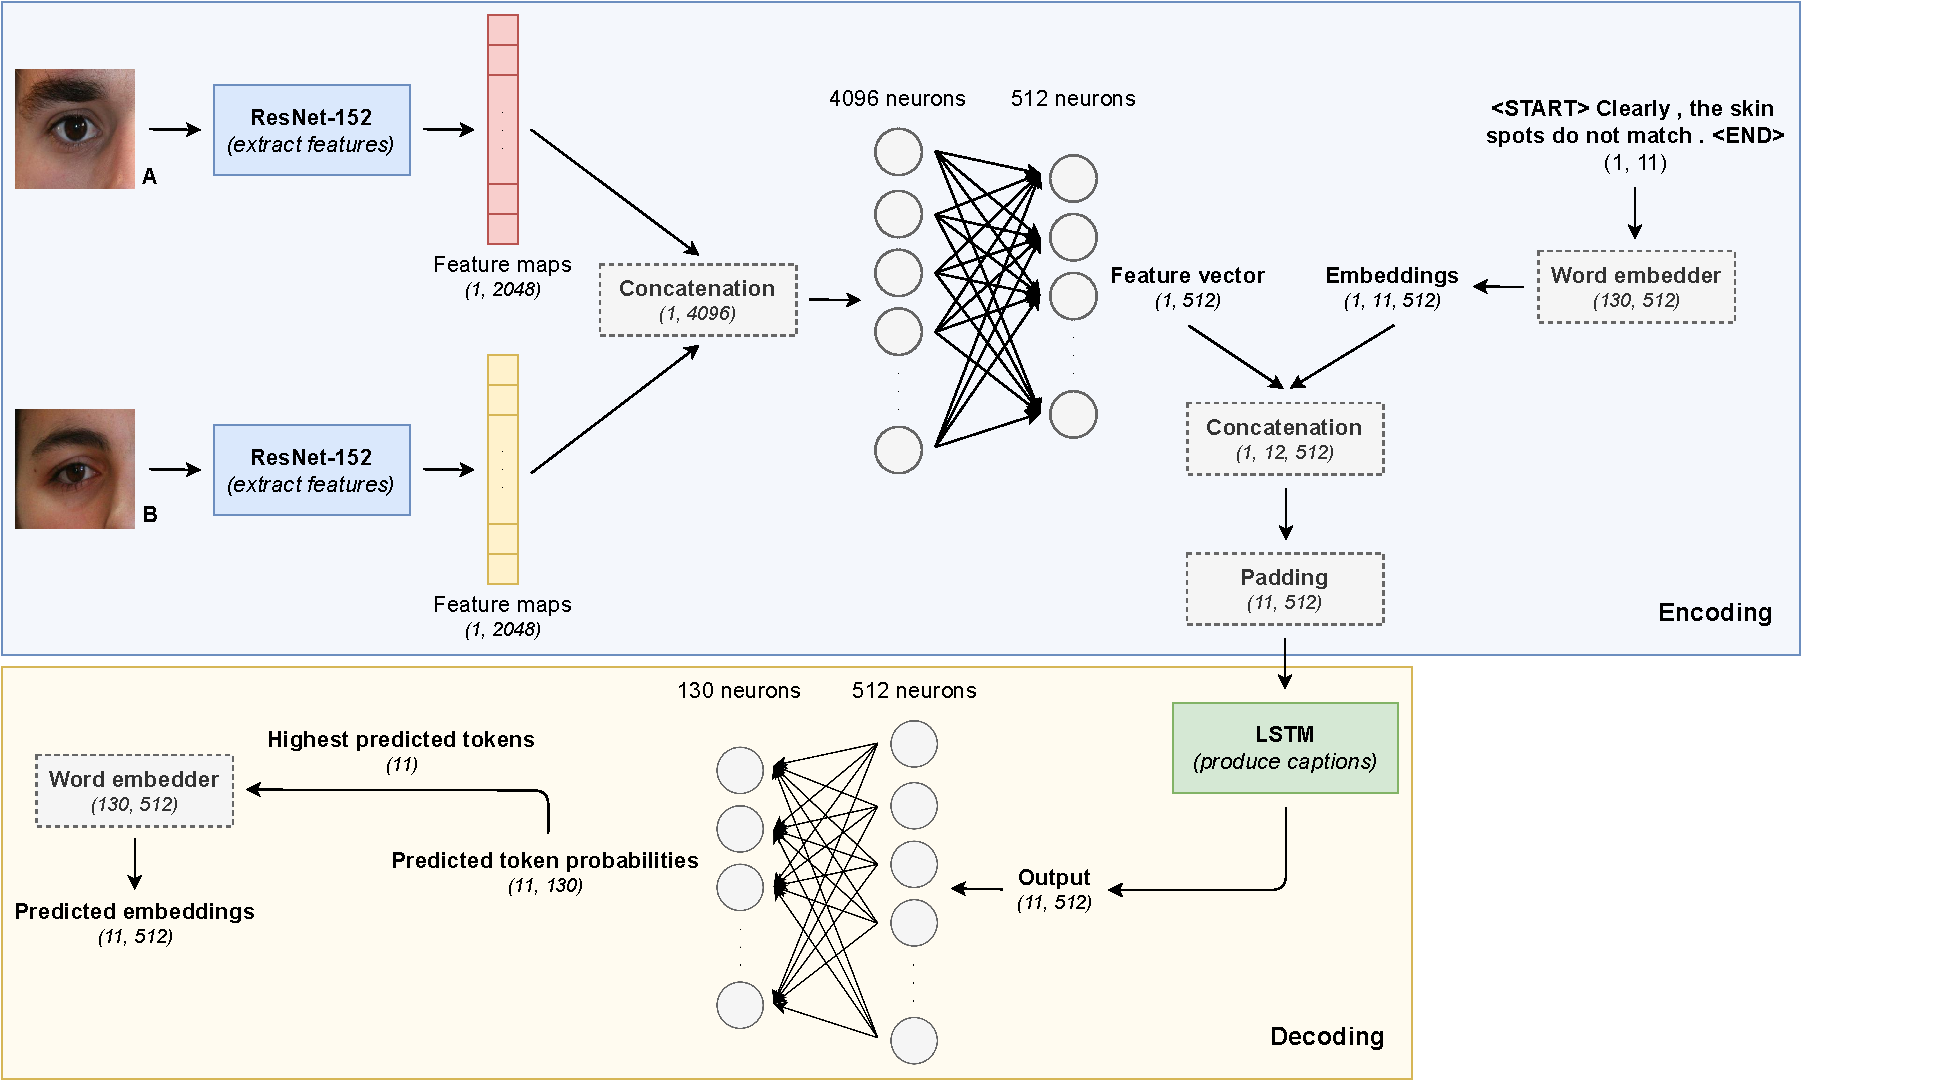
\includegraphics[width=430pt]{figures/figure_30.pdf}
\caption{Overview of the learning stage of the captioning solution. A given image pair is given to the same \ac{CNN}, which extracts a feature map for each image. Then, the two feature maps are concatenated lengthwise and given to a couple of linear layers, culminating in a $512$-dimensional feature vector. At the same time, the ground-truth caption is embedded and concatenated with the feature vector, leading the resulting tensor through a padding operation (to ensure consistency). Next, the \ac{LSTM} receives the padded tensor and tries to output the most likely tokens (that make up a caption). Finally, the predicted tokens are encoded so as to retrieve the corresponding embedding, which can naturally be compared to the ground-truth embedding for learning purposes.}
\label{fig:method_b_main_diagram_learning_phase}
\end{figure}

In this architecture, two major components can be considered: an encoder (i.e., the \ac{CNN}) and a decoder (i.e., the \ac{LSTM}). The former tries to produce a compact representation of the images received, while the latter attempts to generate a plausible caption from that representation. More formally, the encoding is done using the ResNet's feature extraction abilities. Firstly, $2048$-dimensional feature maps for both images $A$ and $B$ and concatenated lengthwise to form a single vector with $4096$ values (further compressed into a $512$-dimensional representation with a couple of linear layers). Then, this vector is concatenated with an embedding of the ground-truth caption and sent through a padding operation that rearranges its input to achieve the desired shape.

After these steps, the resulting tensor is fed to the \ac{LSTM}, whose task is to predict the tokens that would make up a realistic caption (after a couple of linear layers). To allow for proper comparison against the ground-truth, the predicted sequence is embedded in a similar fashion as before.

\subsubsection{Inference Phase}
\label{subsec:chap3_method_b_inference_phase}

\begin{figure}[H]
\centering
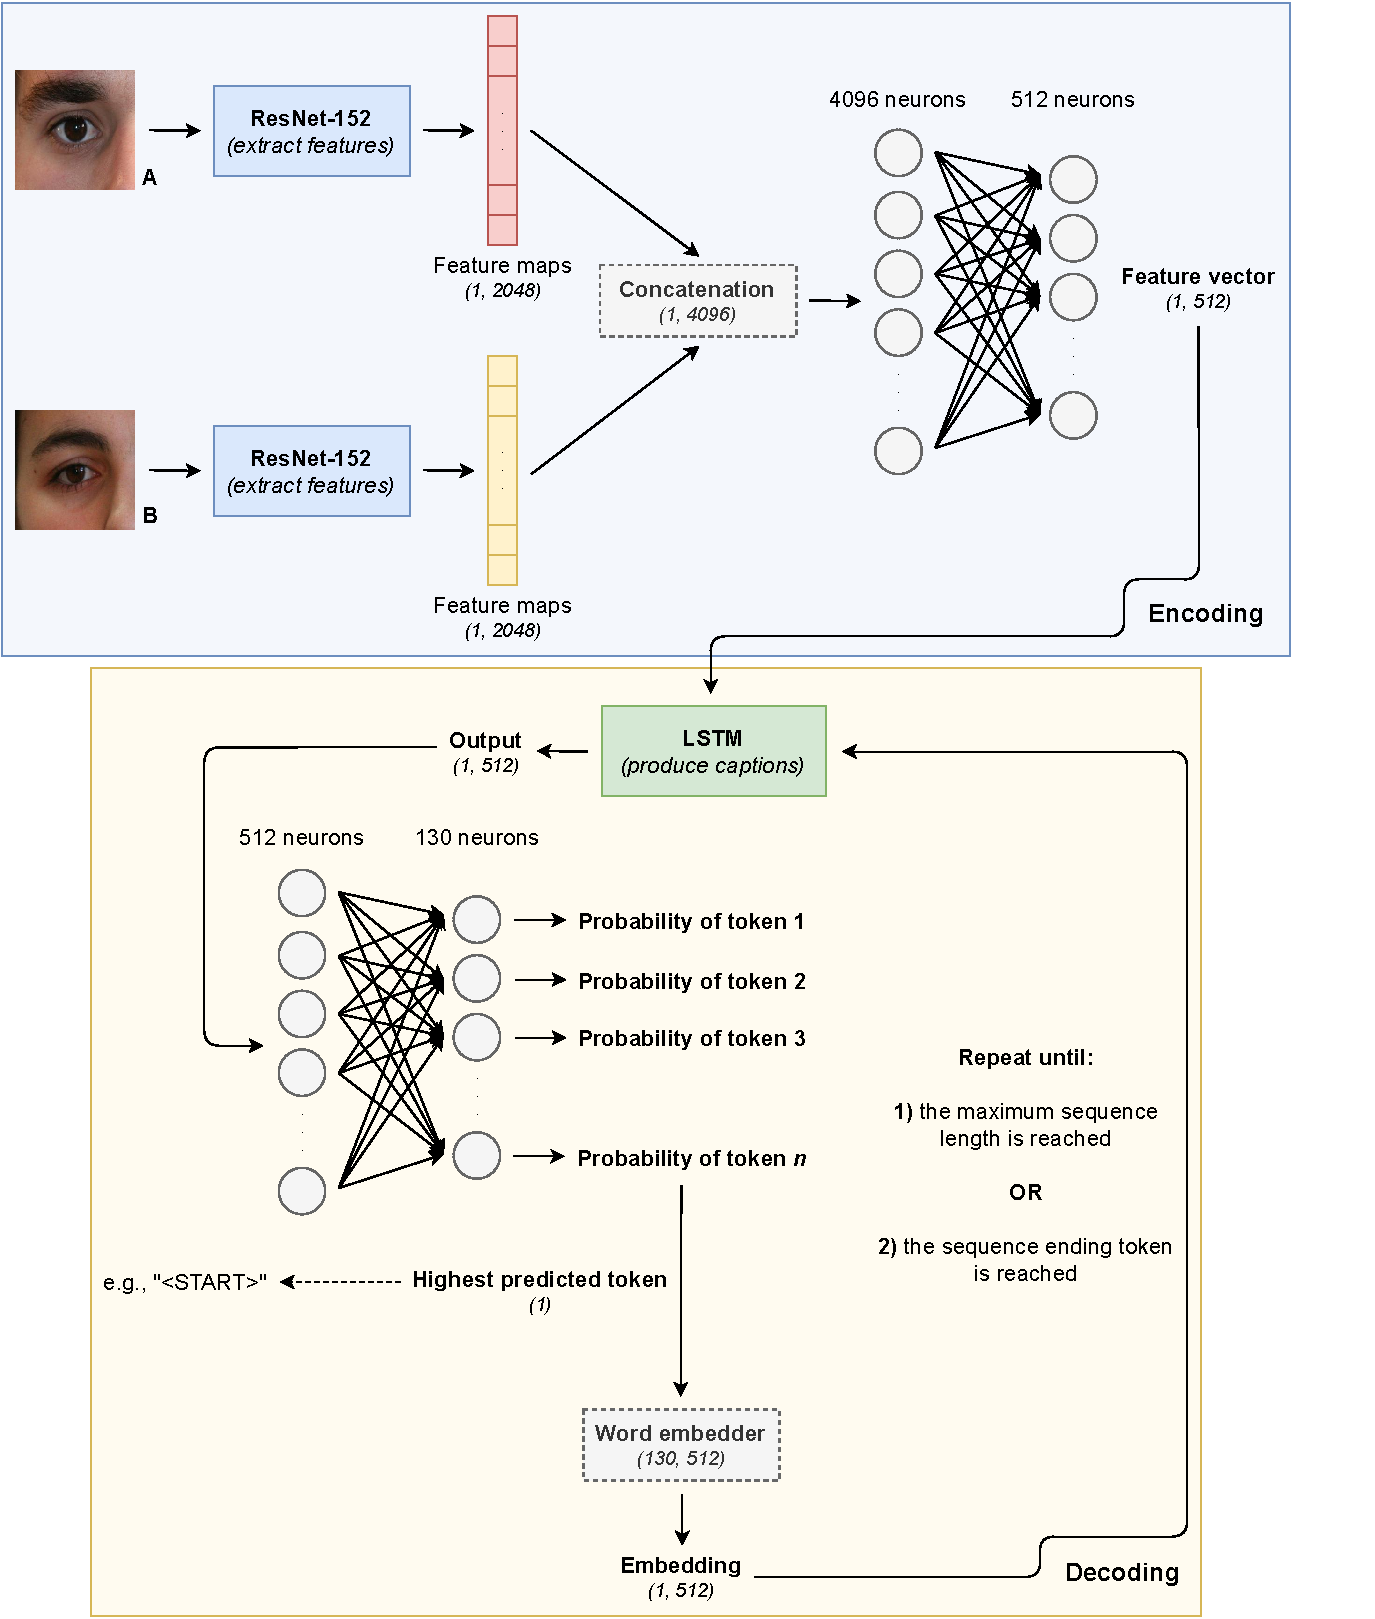
\includegraphics[width=350pt]{figures/figure_31.pdf}
\caption{In inference mode, the encoding stage is kept: two feature maps are derived, concatenated and compressed further into a $512$-dimensional feature vector. Unlike before, the decoding starts with the \ac{LSTM} receiving the feature vector as is and, in conjunction with two linear layers, outputting the most probable token to start a sentence (ideally, "<START>"). The predicted token is fed to the embedder and the resulting representation is fed back to the \ac{LSTM}, completing a loop. To exit said loop, one of two conditions must be met: either the maximum sequence length is reached or the "<END>" token is output.}
\label{fig:method_b_main_diagram_inference_phase}
\end{figure}

Once finished training, the encoding stage remains virtually the same: the two images go through the same \ac{CNN}, the resulting feature maps are concatenated and a couple of linear layers predict a feature vector. It is in the decoding stage that differences start to appear. Firstly, the \ac{LSTM} receives just the feature vector and, with the aid of two linear layers, predicts the first token (ideally, "<START>"). An embedding is derived (as in training) and fed to the \ac{LSTM} so that it contiues the token generation process until we reach one the following stop criteria: $\mathbf{1}$) the predicted sequence reaches a length bigger than the pre-defined maximum or $\mathbf{2}$) the "<END>" token is reached.

\subsection{Implementation Details}
\label{subsec:chap3_method_b_implementation_details}
The method described before was trained for a total of $20$ epochs with a learning rate of $0.001$ and a batch size of $64$ samples. The total number of training samples was roughly $1000$ unique pairs, with each having $2$ available captions (thus equating to approximately $2000$ "pair-caption" combinations). Once again, the Adam optimiser was used to update the weights (with default $\beta_1$ and $\beta_2$ values). Unlike before, the \ac{CNN}'s parameters were not update and instead the ImageNet weights were used. Furthermore, the embedding length was set to $512$, as was the \ac{LSTM}'s hidden size (i.e., the number of units in the unrolled chain).

\section{Conclusion}
\label{sec:chap3_conclusion}

This chapter described the two methods developed to fulfil the proposed goal: being able to explain \textit{why} two images appear to be from different subjects. While the first solution operates in the visual domain (i.e., images), the second method attempts to convey a similar amount of information in written form. Naturally, the next chapter will evaluate these approaches, with a range of samples from each.